\subsection{Data Mapper Pattern}
\label{data_mapper_pattern_section}

Originally, the \emph{Layer PerCom} approach of CYBOP was based on the \emph{Data Mapper} pattern
(figure \ref{fig:DataMapper}).
\begin{figure}[ht]
    \begin{center}
       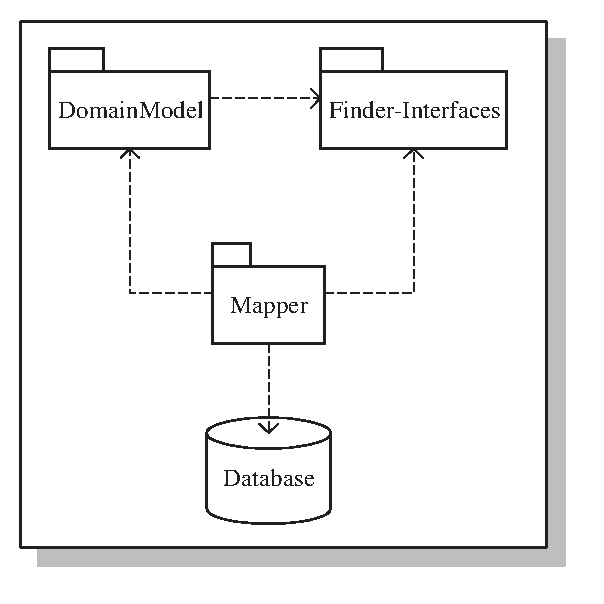
\includegraphics[scale=0.6]{images/data_mapper_pattern.eps}
       \caption{The Data Mapper - Pattern \cite{enterprisepattern}}
       \label{fig:DataMapper}
    \end{center}
\end{figure}

It is part of Martin Fowler's pattern collection called \emph{Enterprise Application Architecture}
\cite{enterprisepattern}. The most important idea of this pattern is
to abolish the interdependency of domain model and database (persistence).\\
The arrows in figure \ref{fig:DataMapper} indicate the direction of dependency.
Each domain model class knows its appropriate persistence finder interface but
does not know their implementation, i.e. how data are actually retrieved from
the database. The data mapper implementation is part of the mapping package
that implements all finders and maps all data of the received result set to the
special attributes of the domain model objects.\\
There is no need for the domain model to know where the database is located or how
to get the data -- and also not how to map the entity-relationship model data.
If all these things are done by the corresponding data mappers, why shouldn't
it be possible to get such a mapping package for persistence media of any kind,
no matter which communication paradigm (File Stream, JDBC, ODBC with SQL) is used?
Users would have a number of persistence mechanisms to dynamically choose from;
Developers would not have to implement the same mechanisms again and again for
each new Module (Application) -- leading to clearer code with greatly reduced size.\\
This functional code separation would make it very easy to develop a complicated
domain model and update it later, if necessary. The data mapper package could
contain special parts for local storage in a file system, in various file formats
such as XML, CSV, RTF, TXT etc. (whether it makes sense or not to store domain data
in a pure text file), for a number of databases (relational, object relational,
object oriented) and so on.
Each of those specialised parts knows how to communicate with its appropriate
persistence medium and only with it. They all include a specialised mapper class,
called \emph{Translator} in CYBOP. It translates the data from the domain model
to the model of the corresponding persistence mechanism.\\
